\documentclass[]{article}

\usepackage{polski}
\usepackage[utf8]{inputenc}
\usepackage{graphicx}
\usepackage{float}
\usepackage{url}
\usepackage[T1]{fontenc}
\usepackage{beramono}
\usepackage{listings, lstautogobble}
\usepackage{xcolor}
 
\lstdefinelanguage{VHDL}{
   morekeywords={
     library,use,all,entity,is,port,in,out,end,architecture,of,
	 begin,and,impure,function,file,variable,for,loop,readline,read,
	 return,signal,bit_vector,open,if,else,elsif,then,or,downto,process,
	 unsigned,std_logic_vector
   },
   morecomment=[l]--
}
\colorlet{keyword}{blue!100!black!80}
\colorlet{comment}{green!70!black!80}
\lstdefinestyle{vhdl}{
   language     = VHDL,
   basicstyle   = \scriptsize\ttfamily,
   keywordstyle = \color{keyword}\bfseries,
   commentstyle = \color{comment}
}

\title{Obsługa wyświetlacza OLED z wykorzystaniem układu z rodziny Spartan-3E}
\date{22-05-2019}
\author{
	Marcin Wojciechowski \\
	Tobiasz Rumian \\ \\
	Prowadzący: dr inż. Jarosław Sugier
}

\begin{document}
	\pagenumbering{gobble}
	\maketitle
	\newpage
	\tableofcontents
	\newpage
	\pagenumbering{arabic}

	\section{Wstęp}
	\subsection{Cel i zakres projektu}
	Zamierzonym efektem finalnym projektu jest stworzenie 4 cyfrowego licznika, zwiększającego się za każdym wciśnięciem przycisku klawiatury. Do obsługi wyświetlacza OLED128x64 wykorzystany będzie układ Spartan-3E FPGA. Klawiatura podłączona będzie poprzez port PS/2 do wspomnianym wyżej urządzenia.\\
	Pracę została podzielona na pomniejsze etapy:
	\begin{enumerate}
		\item Stworzenie map bitowych cyfr do wyświetlenia
		\item Wczytanie powyższych map do pamięci urządzenia
		\item Wyświetlenie liczb na wyświetlaczu
		\item Dołączenie do schematu modułu PS/2
		\item Zmiana wypisywanych liczb poprzez wciśnięcie przycisku klawiatury
	\end{enumerate}
	
	\subsection{Opis sprzętu}
	\subsubsection{Układ Spartan-3E FPGA Starter Kit}
	Układ Spartan-3E wyposażony jest w układ FPGA Spartan-3E 500K z 32-bitowym procesorem RISC oraz interfejsami DDR. Najważniejszym aspektem przy naszym projekcie jest możliwość podłączenia urządzenia peryferyjnego, poprzez jedno z trzech 6-pinowych połączeń, oznaczonych jako J1, J2 oraz J4. \cite{ug230}
	\begin{figure}[H]
		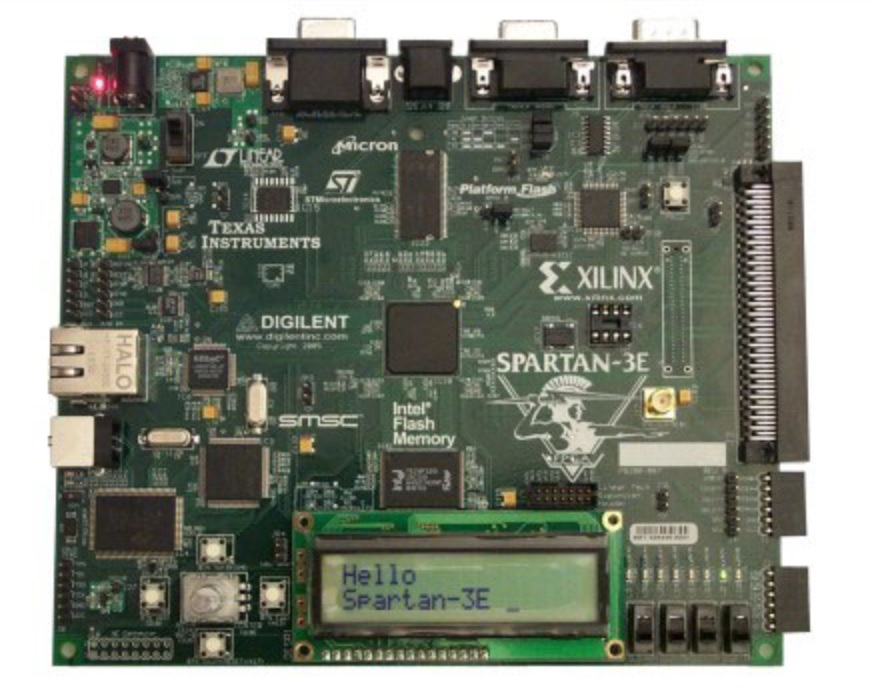
\includegraphics[width=.7\linewidth]{img/spartan.jpg}
		\centering
		\caption{Układ Spartan-3E FPGA Starter Kit}
		\label{fig:spartan}
	\end{figure}
	\subsubsection{Wyświetlacz OLED128x64 ze sterownikiem SSD1306}
	Do wyświetlania liczb na ekranie wykorzystany został wyświetlacz OLED128x64 z jednoukładowym sterownikiem SSD1306 do wyświetlania graficznego na matrycy punktowej, zaprojektowanego do pracy z panelem OLED typu Common Cathode o wymiarach 128x64. Kontrola urządzenia odbywa się poprzez interfejs równoległy, interfejs I2C lub interfejs szeregowy peryferyjny. Możliwe jest również sterowanie jasnością wyświetlacza w zakresie 0-256, jednak projekt nie obejmuje kontroli tego ustawienia. Do komunikacji wykorzystany zostanie interfejs I2C. \cite{oled}
	\begin{figure}[H]
		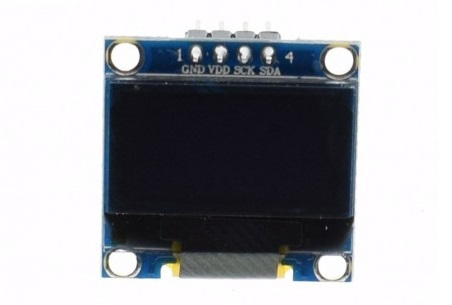
\includegraphics[width=.3\linewidth]{img/oled.jpg}
		\centering
		\caption{Wyświetlacz OLED128x64 SSD1306}
		\label{fig:oled}
	\end{figure}
	
	\subsection{Środowisko}
	Program obsługujący zachowania urządzeń został napisany w języku VHDL, wykorzystując środowisko do syntezy układów Xilinx ISE. \\
	To środowisko oferuje syntezę HDL, symulacje oraz implementacje układów, w związku z czym to właśnie z tego programu pochodzą zamieszczone zrzuty ekranu.

	\subsection{Opis interfejsów i używanych protokołów}
	\subsubsection{Magistrala I2C}
	I2C (zwana również jako Inter IC) to szeregowa, dwukierunkowa magistrala pozwalająca na wydajną kontrolę pomiędzy układami scalonymi. Stała się światowym standardem, który jest wdrażany w nowych układach scalonych produkowanych w różnych firmach. Dzięki temu konceptowi, możliwe jest przesyłanie danych za pomocą jedynie dwóch linii magistrali - szeregowej danych (SDA) oraz szeregowej zegarowej (SCL). \cite{i2c}
	\subsubsection{Port komunikacyjny PS/2}
	Interfejs PS/2, opracowany przez IBM, był swego czasu używany przez wiele myszy i klawiatur. Jest to 5-pinowy port zapewniający zasilanie oraz komunikację między komputerem a klawiaturą. \cite{ps/2}


	\section{Opis projektu}
	\subsection{Schemat główny}
	Na Rysunku \ref{fig:top} przedstawiony został głowny schemat naszego projektu. Korzysta on z 5 sygnałów wejściowych:
	\begin{itemize}
		\item PS2\_Clk - zegar do modułu obsługującego port PS2,
		\item PS2\_Data - dane wejściowe klawiatury,
		\item Clk - 50MHz zegar procesora,
		\item Reset - umożliwiający resetowanie modułów układu,
		\item Wartość stała 78 - oznaczająca adres urządzenia połączonego przez magistralę I2C,
	\end{itemize}
	1 sygnału wyjściowego - LED7 - okazujący brak potwierdzenia odbioru bajtu przez urządzenie , oraz 2 sygnałów dwukierunkowych - SDA oraz SCL, odpowiadające liniom magistralii I2C
	\begin{figure}[H]
		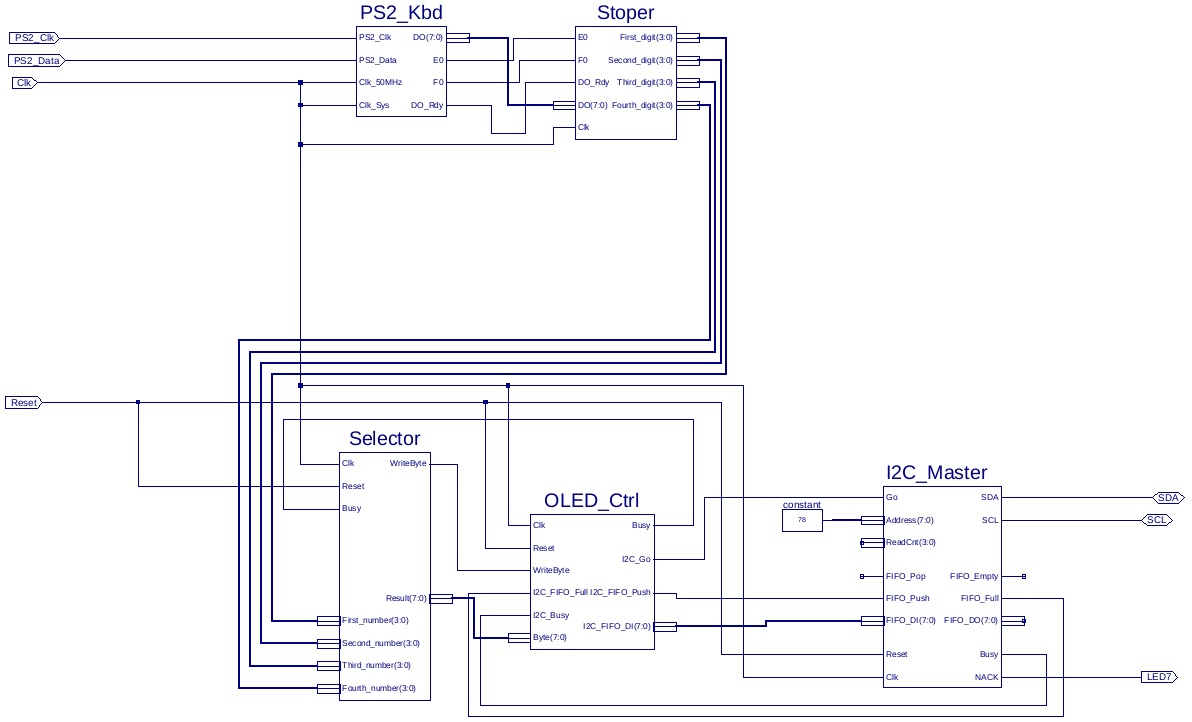
\includegraphics[width=\linewidth]{img/top.jpg}
		\caption{Schemat główny układu}
		\label{fig:top}
	\end{figure}
	W projekcie korzystamy z kilku gotowych modułów stworzonych przez dr inż. Jarosława Sugier. Moduł I2C\_Master jest modułem sterownika magistrali I2C w trybie Fast-mode (400kbps) z 16B kolejką FIFO na buforowanie przekazywanych danych. Moduł PS2\_Kbd jest odbiornikiem kodów wysyłanych przez klawiaturę podłączoną przez port PS/2. Moduł OLED\_Ctrl jest automatem skończonym, który wykonuje inicjalizację wyświetlacza \cite{fpga}. W dokumentacji zostaną omówione moduły w których musieliśmy wprowadzić zmiany, aby dopasować dany symbol do naszego projektu. 
	
	\subsection{Hierarchia projektu}
	\begin{figure}[H]
		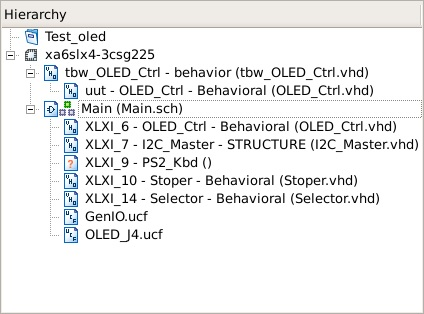
\includegraphics[width=\linewidth]{img/hierarchy.jpg}
		\caption{Hierarchia projektu}
		\label{fig:hierarchy}
	\end{figure}
	
	\subsection{Opisy szczegółowe modułów}
	\subsubsection{Moduł OLED\_Ctrl}
	\begin{figure}[H]
		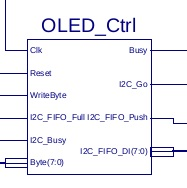
\includegraphics[width=.4\linewidth]{img/oled_ctrl.jpg}
		\centering
		\caption{Moduł OLED\_Ctrl}
		\label{fig:oledctrl}
	\end{figure}
	Aby łatwiej przesyłać cyfry do sterownika SSD1306, w tablicy inicjalizującej wyświetlacza zmieniony został tryb adresowania na pionowy, co umożliwi wysyłanie cyfr po kolei, zamiast mieszania ich poziomych fragmentów.
	\noindent\begin{lstlisting}[style=vhdl, autogobble=true, label={lst:mem}, caption={Funcja inicjalizacji pamięci w module Selector}, captionpos=b]
		constant ROM : t_byte_array( 0 to ARR_LEN - 1 ) := ( 
			-- Minimal initialization command bytes:
			X"00",            -- string prefix: commands (not data) will follow
			X"A1", X"C8",     -- set segment remap & reverse COM output scan direction
			X"20", X"01",     -- set vertical addressing mode
			X"8D", X"14",     -- enable charge pump
			X"AF"             -- set display ON
		);
	\end{lstlisting}

	\subsubsection{Moduł Stoper}
	\begin{figure}[H]
		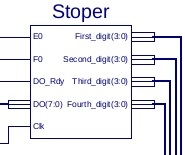
\includegraphics[width=.5\linewidth]{img/stoper.jpg}
		\centering
		\caption{Moduł Stoper}
		\label{fig:stoper}
	\end{figure}
	Moduł zawiera następujące wejścia:
	\begin{itemize}
		\item E0 - niepotrzebne?
		\item F0 - niepotrzebne?
		\item DO\_Rdy - sygnał jednotaktowy przekazany z modułu PS2\_Kbd, sygnalizujący zakończenie odbioru kodu z klawiatury
		\item DO(7:0) - wartość kodu klawiatury z modułu PS2\_Kbd,
		\item Clk - zegar procesora
	\end{itemize}
	oraz wyjścia:
	\begin{itemize}
		\item First\_digit(3:0),
		\item Second\_digit(3:0),
		\item Third\_digit(3:0),
		\item Fourth\_digit(3:0),
	\end{itemize}
	gdzie każde z nich oznacza jedną z cyfr (0-9) do wyświetlenia.
	Moduł składa się z czterech liczników modulo 10 - pierwsza cyfra jest inkrementowana przez wciśnięcie klawisza na klawiaturze, a każde wyzerowanie cyfry powoduje zwiększenie kolejnej.
	\noindent\begin{lstlisting}[style=vhdl, autogobble=true, label={lst:stoper}, caption={Proces licznika w module stoper}, captionpos=b]
		process1 : process( Clk, started )
		begin
		if rising_edge( Clk ) and started='1' then
		   if First_counter="1010" then
			  First_counter<="0000";
			  Second_counter<=std_logic_vector( unsigned(Second_counter) + 1 );
		   end if;
		   if Second_counter="1010" then
			  Second_counter<="0000";
			  Third_counter<=std_logic_vector( unsigned(Third_counter) + 1 );
		   end if;
		   if Third_counter="1010" then
			  Third_counter<="0000";
			  Fourth_counter<=std_logic_vector( unsigned(Fourth_counter) + 1 );
		   end if;
		   if Fourth_counter="1010" then
			  Fourth_counter<="0000";
		   end if;
		   if clk_counter=X"02FAF080" then 
			  clk_counter<=X"00000001";
			  First_counter<=std_logic_vector( unsigned(First_counter) + 1 );
		   else
			  clk_counter<=std_logic_vector( unsigned(clk_counter) + 1 );
		   end if;
		end if;
		end process process1;
	\end{lstlisting}

	\subsubsection{Moduł Selector}
	\begin{figure}[H]
		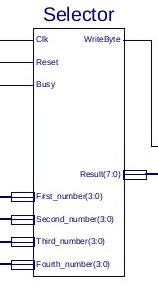
\includegraphics[width=.4\linewidth]{img/selector.jpg}
		\centering
		\caption{Moduł Selector}
		\label{fig:selector}
	\end{figure}
	Moduł zawiera następujące wejścia:
	\begin{itemize}
		\item Clk - zegar procesora
		\item Reset - przycisk reset
		\item Busy - zaznacza, że moduł OLED\_Ctrl otrzymał już bajt i należy poczekać przed wysłaniem kolejnego
		\item First\_number(3:0), Second\_number(3:0), Third\_number(3:0),\\ Fourth\_number(3:0) - liczby wychodzące z modułu stoper
	\end{itemize}
	oraz następujące wyjścia:
	\begin{itemize}
		\item WriteByte - oznaczający gotowość do wysłania bajtu
		\item Result - fragment mapy bitowej cyfr (bajt)
	\end{itemize}
	Ten moduł odpowiada za wczytanie do pamięci przygotowanych przez map bitowych cyfr w postaci plików .MIF poprzez funkcję init\_mem pokazaną w Listingu \ref{lst:mem}. Kolejną kluczową odpowiedzialnością tego modułu, jest wysyłanie do sterownika wyświetlacza OLED odpowiednich cyfr, bajt po bajcie (proces pokazany w Listingu \ref{lst:send}).

	\noindent\begin{lstlisting}[style=vhdl, autogobble=true, label={lst:mem}, caption={Funcja inicjalizacji pamięci w module Selector}, captionpos=b]
		impure function init_mem(mif_file_name : in string) return mem_type is
			file mif_file : text open read_mode is mif_file_name;
			variable mif_line : line;
			variable temp_bv : bit_vector(DATA_WIDTH-1 downto 0);
			variable temp_mem : mem_type;
		begin
			for i in mem_type'range loop
				readline(mif_file, mif_line);
				read(mif_line, temp_bv);
				temp_mem(i) := to_stdlogicvector(temp_bv);
			end loop;
			return temp_mem;
		end function;
	\end{lstlisting}
	\noindent\begin{lstlisting}[style=vhdl, autogobble=true, label={lst:send}, caption={Proces wysyłający mapy bitowe cyfr do sterownika w module Selector}, captionpos=b]
		process1 : process( Clk )
		begin
		   if rising_edge( Clk ) then
			  if Busy = '1' then
				 WriteByte<='0';
				 writeByteBusy<='0';
			  end if;
			  if lineNumber=32 then
				 lineNumber<=0;
			  end if;
			  if Reset = '1' then
				 state <= WRITE_FIRST;
			  else
				 state <= next_state;
			  end if;
			  if (Busy= '0') and (
				  state = WRITE_FIRST or 
				  state = WRITE_SECOND or 
				  state = WRITE_THIRD or 
				  state = WRITE_FOURTH) and 
				  blockNumber<8 and 
				  lineNumber<IMAGE_SIZE and 
				  writeByteBusy='0' then
				chunk <= tmpBitmap(lineNumber)(7+8*blockNumber downto 8*blockNumber);
				blockNumber<=blockNumber+1;
				WriteByte<='1';
				writeByteBusy<='1';
				if blockNumber = 7 then
					blockNumber<=0;
					lineNumber<=lineNumber+1;
				 end if;
			  end if;
		   end if;
		end process process1;
	\end{lstlisting}

	\section{Symulacje}
	\subsection{Symulacja modułu...}
	Fotka z symulacji
	
	
	\section{Implementacja}
	\subsection{Podsumowanie generowania pliku programowego}
	Na układzie wykorzystujemy około 244 przerzutników, co stanowi około 2\% spośród wszystkich dostępnych na urządzeniu. (Rysunek \ref{fig:summary})
	\begin{figure}[H]
		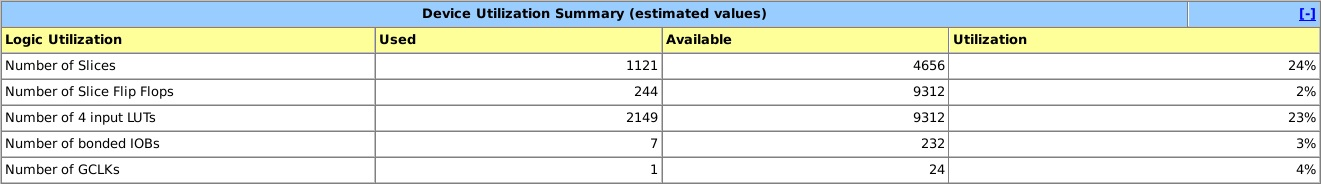
\includegraphics[width=\linewidth]{img/design_summary.jpg}
		\caption{Podsumowanie generowania pliku programowego}
		\label{fig:summary}
	\end{figure}
	
	\subsection{Zależności czasowe projektu}
	Z zależności czasowych stworzonych podczas kompilacji można zauważyć, że mieścimy się w jednym okresie 50MHz zegara procesora - 16.122/20 ns(Rysunek \ref{fig:time})
	\begin{figure}[H]
		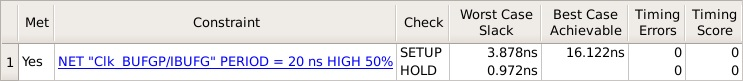
\includegraphics[width=\linewidth]{img/time_constraints.jpg}
		\caption{Zależności czasowe projektu}
		\label{fig:time}
	\end{figure}
	
	\subsection{Podręcznik użytkowania}
	W celu uruchomienia projektu, należy podłączyć urządzenia w sposób pokazany na Rysunku \ref{fig:all}. Klawiaturę należy podłączyć poprzez port PS/2 (również widoczny na Rysunku \ref{fig:all} - fioletowa wtyczka z tyłu urządzenia). Wyświetlacz należy podpiąć do 6-pinowego połączenia do modułów peryferyjnych, oznaczonego na układzie jako J4) - przybliżenie połączenia zostało pokazane na Rysunku \ref{fig:j4}.
	\begin{figure}[H]
		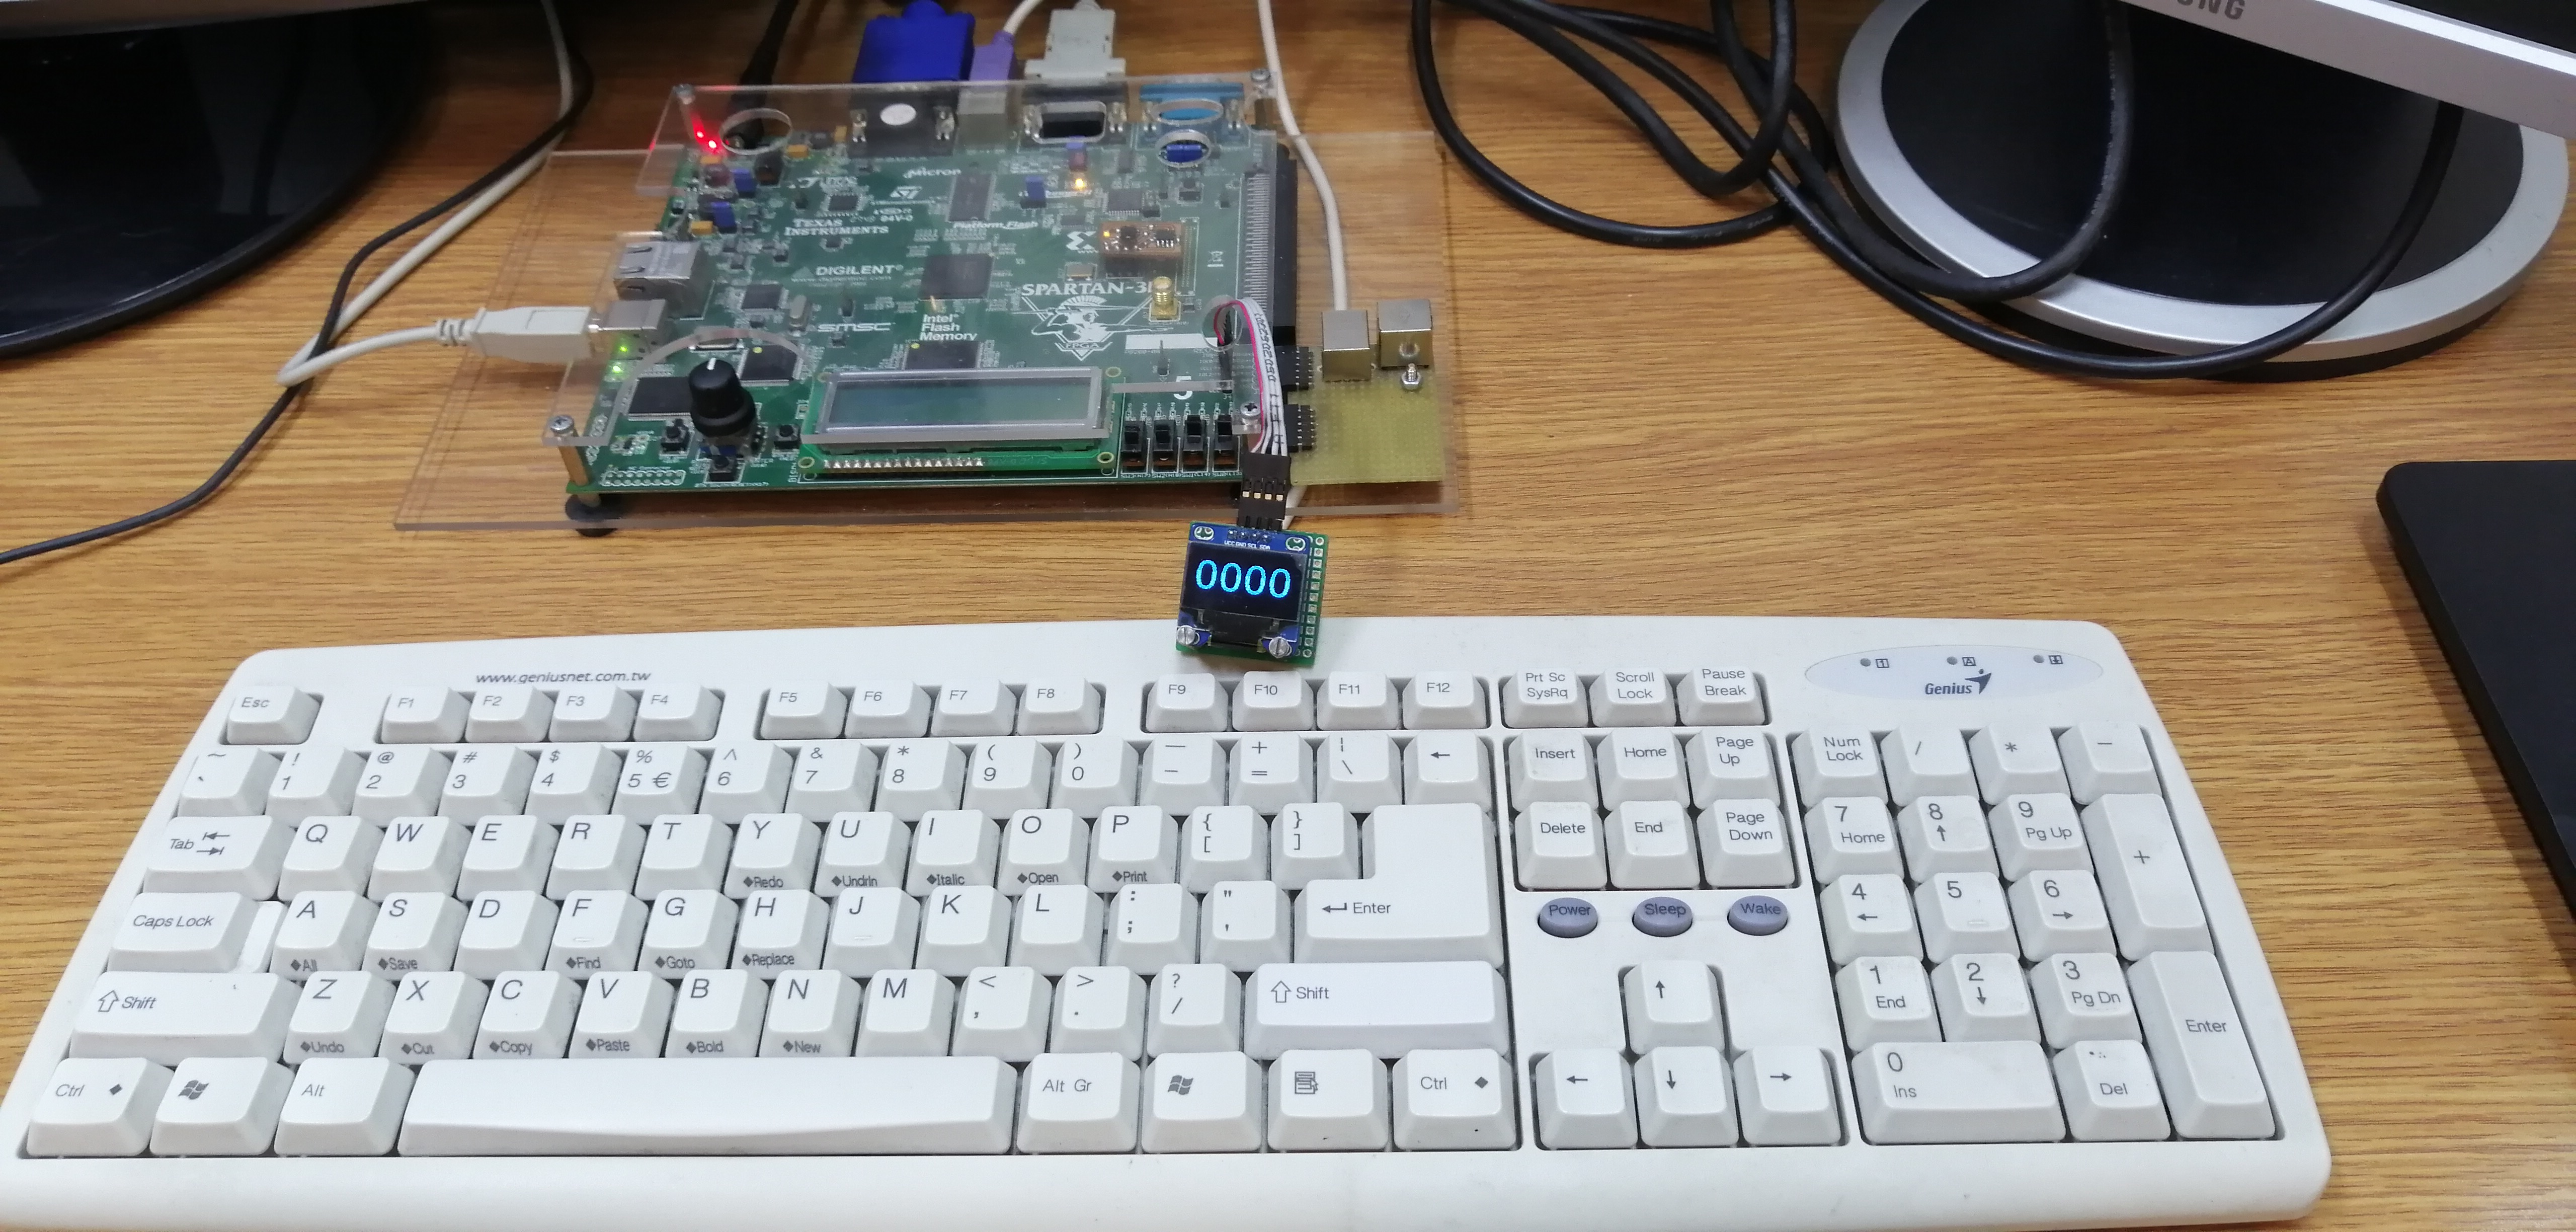
\includegraphics[width=\linewidth]{img/all.jpg}
		\caption{Pełne połączenie schematu}
		\label{fig:all}
	\end{figure}
	\begin{figure}[H]
		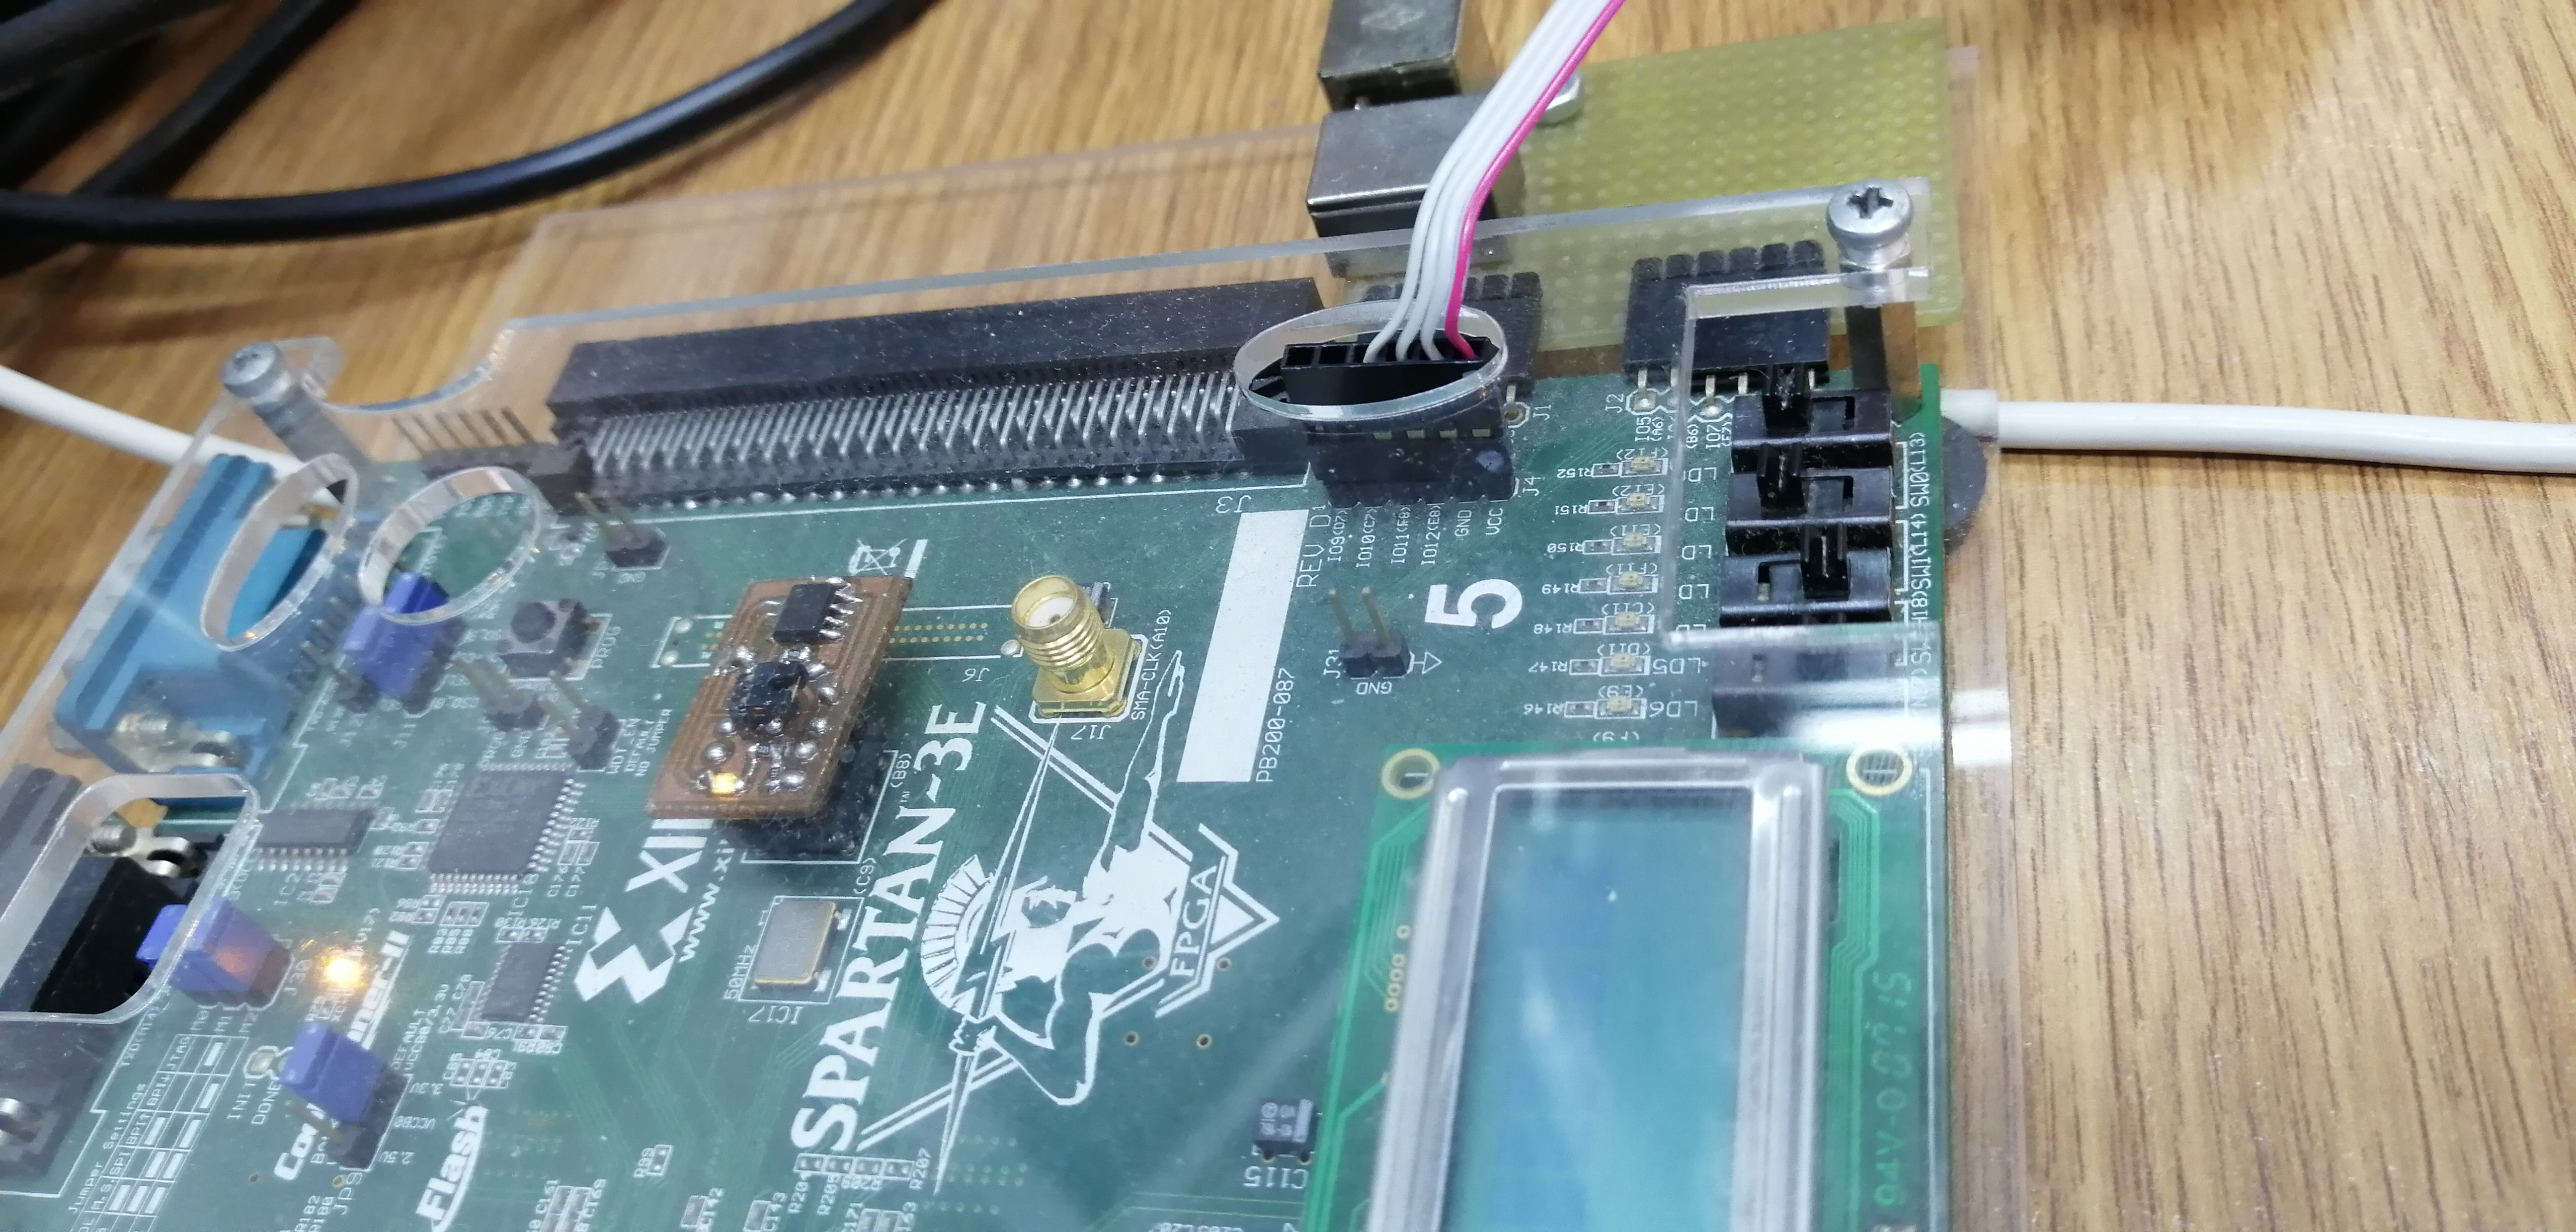
\includegraphics[width=\linewidth]{img/connection.jpg}
		\caption{Połączenie układu Spartan z wyświetlaczem}
		\label{fig:j4}
	\end{figure}
	Efekt działania programu widoczny jest na wyświetlaczu OLED - licznik jest zwiększany poprzez wciśnięcie klawisza spacja na klawiaturze (Rysunek \ref{fig:result}).
	\begin{figure}[H]
		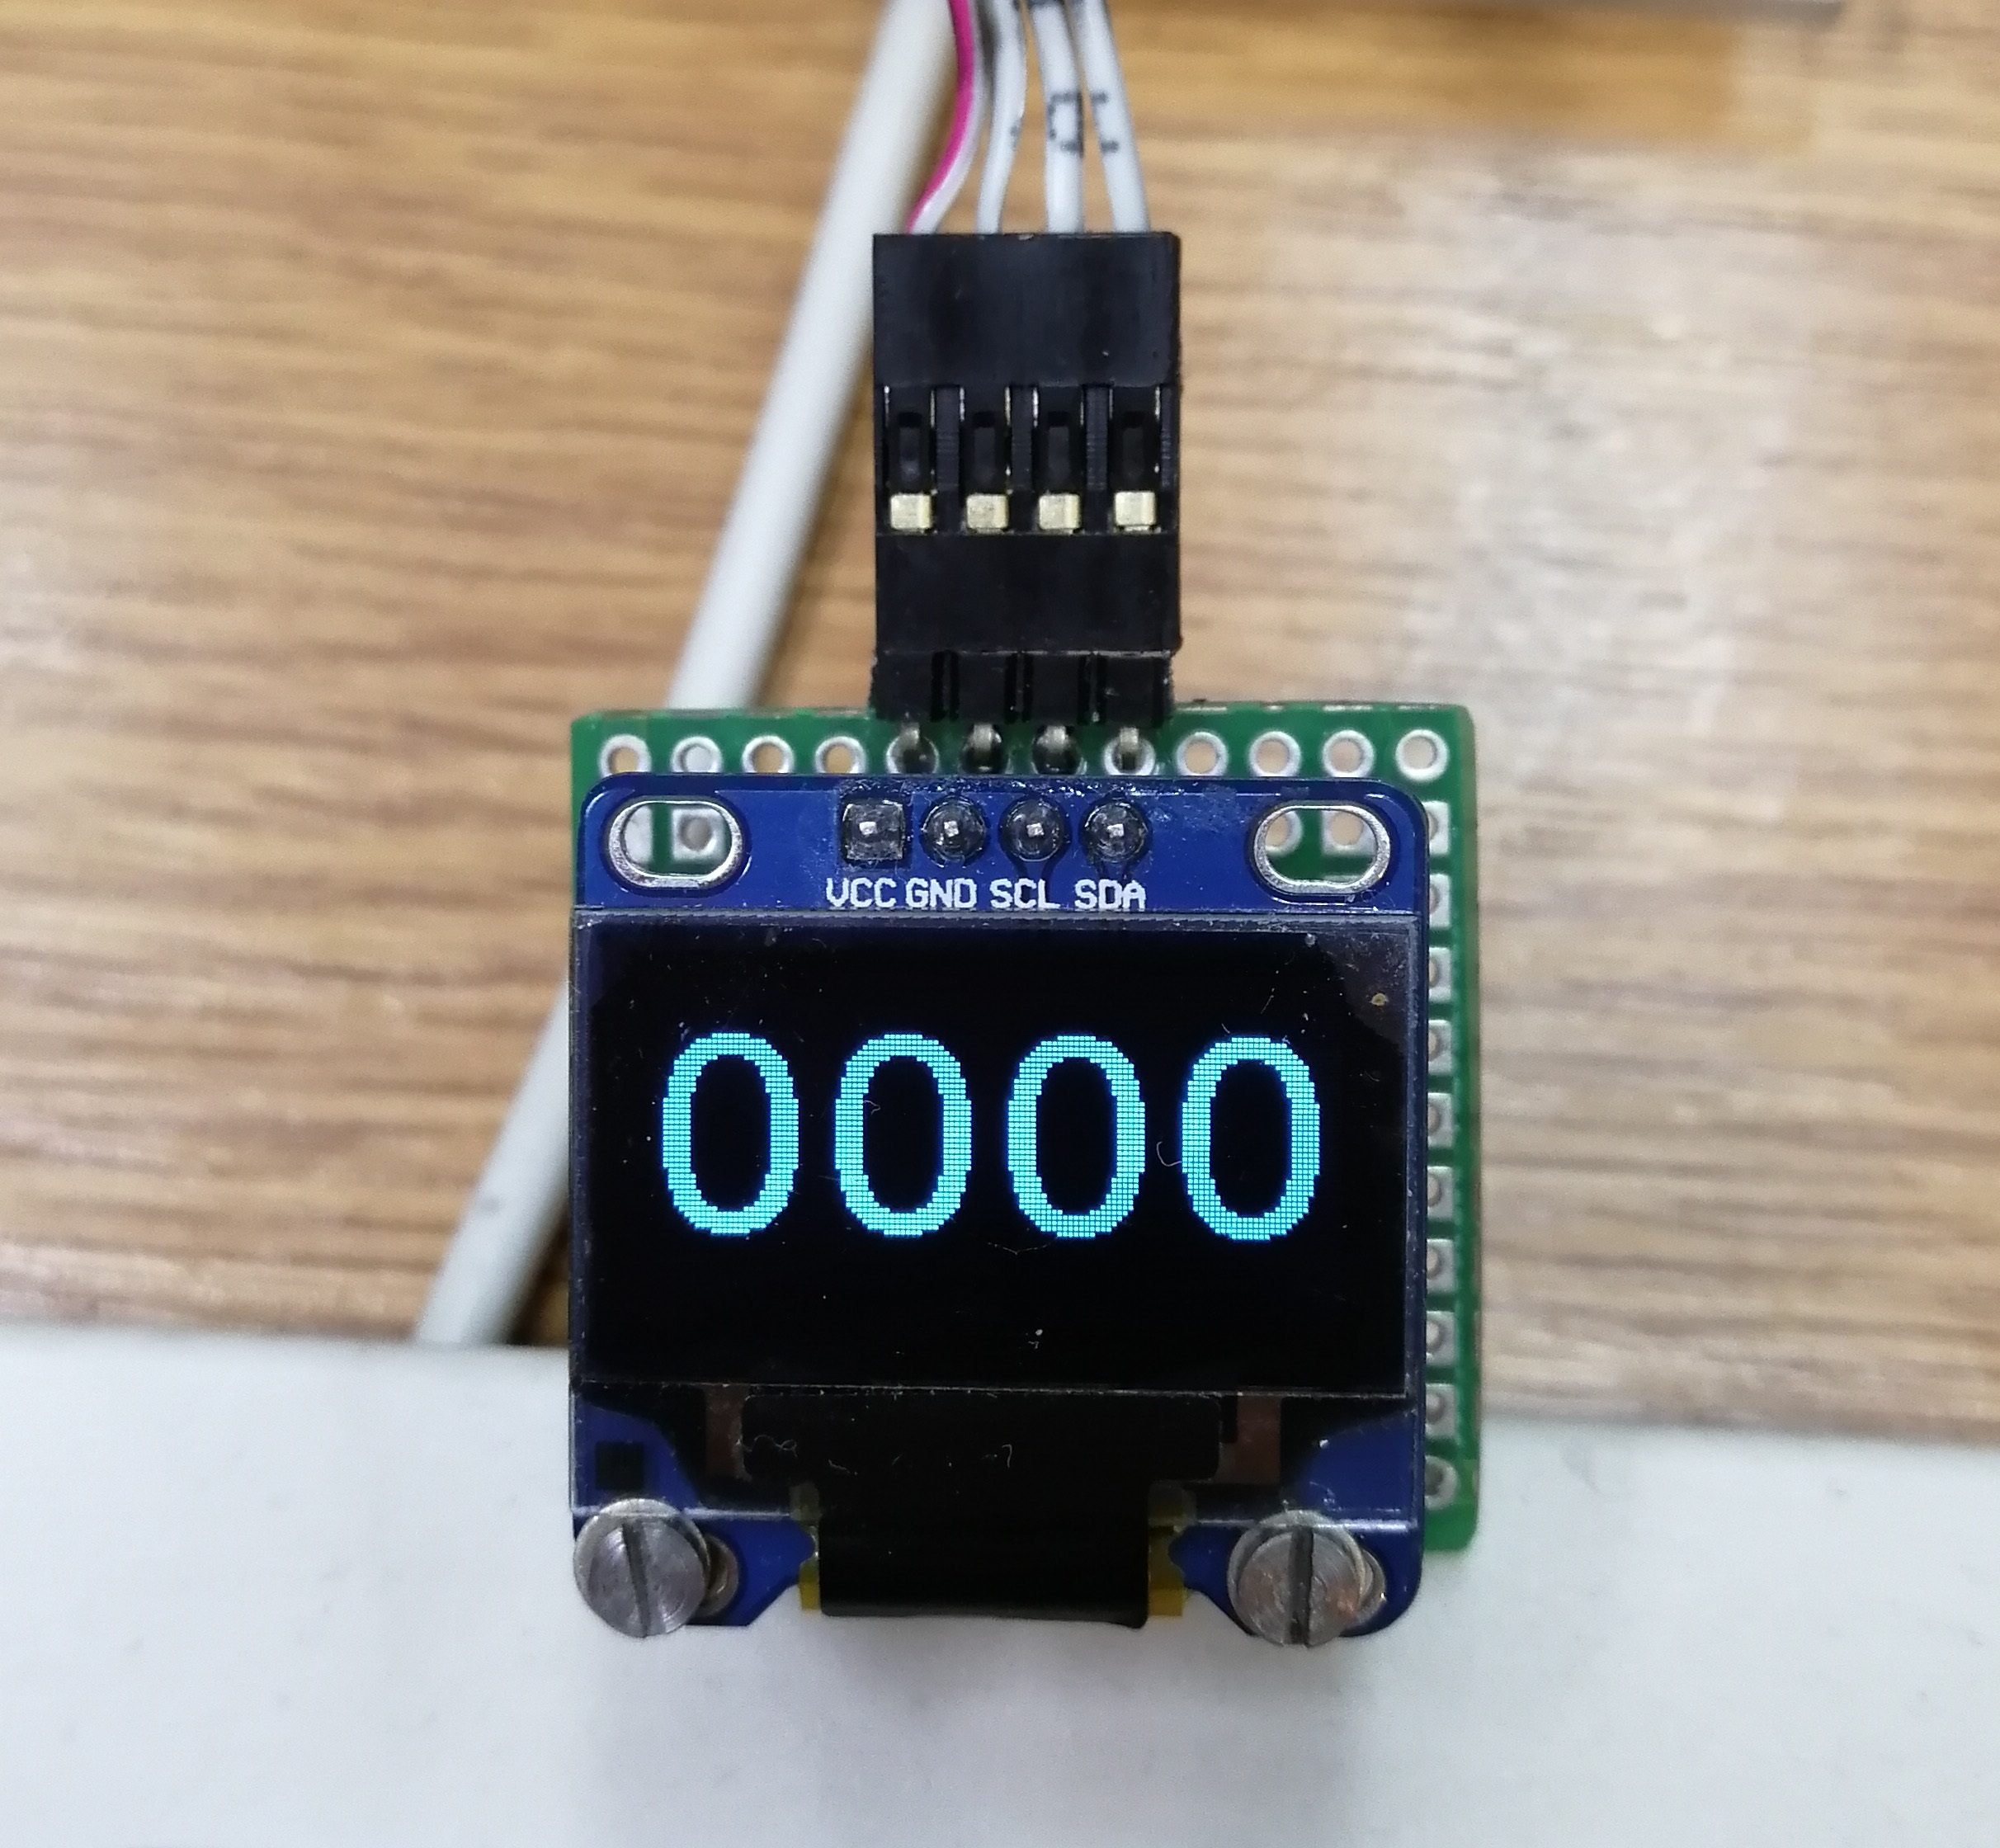
\includegraphics[width=.5\linewidth]{img/result.jpg}
		\centering
		\caption{Efekt działania projektu}
		\label{fig:result}
	\end{figure}

	
	\section{Podsumowanie}
	\subsection{Ocena krytyczna}
	Podczas pracy napotkaliśmy wiele problemów. Największe trudności napotkaliśmy podczas prób wgrania map bitowych liczb układu Spartan. Przygotowane przez nas pliki początkowo nie były poprawnie zapisywane w pamięci, a gdy już udało nam się naprawić ten problem - nie były poprawnie wyświetlane na ekranie. Dopiero po dziewięciu godzinach prób zwalczania błędów oraz kilku korektach liczb ujrzeliśmy na ekranie pierwszą poprawnie wyświetloną cyfrę. Kolejny etap, czyli zmiana cyfr poprzez wciśnięcie klawisza na klawiaturze, również nie przebiegł bez kłopotów. Urządzenie w żaden sposób nie reagowało na podany sygnał wejściowy, co skutkowało spędzeniem kolejnych kilku godzin w symulatorze układu. Ostatecznie, po upartej pracy w domu, % TODO koniec
	
	\subsection{Dalsza praca}
	Nasza praca stanowi dobrą podstawę do dalszej rozbudowy. Mogłaby być ona bazą dla np. stopera aktywowanego poprzez klawiaturę lub budowę zegarka cyfrowego, wystarczyłoby stworzyć odpowiedni układ przeliczający zegar urządzenia na sekundy. 
	
	\subsection{Wnioski}
	Realizacja projektu pokazała nam, w jaki sposób możemy niskopoziomowo komunikować się pomiędzy urządzeniami peryferyjnymi. Problemy które napotkaliśmy rozwinęły nasze umiejętności pracy z symulacjami, bez których bardzo ciężko byłoby znaleźć popełnione przez nas błędy.
	\newpage
	\bibliography{bibliography}
	\bibliographystyle{ieeetr}
\end{document}